% Options for packages loaded elsewhere
\PassOptionsToPackage{unicode}{hyperref}
\PassOptionsToPackage{hyphens}{url}
\PassOptionsToPackage{dvipsnames,svgnames,x11names}{xcolor}
%
\documentclass[
  10pt,
]{article}

\usepackage{amsmath,amssymb}
\usepackage{iftex}
\ifPDFTeX
  \usepackage[T1]{fontenc}
  \usepackage[utf8]{inputenc}
  \usepackage{textcomp} % provide euro and other symbols
\else % if luatex or xetex
  \usepackage{unicode-math}
  \defaultfontfeatures{Scale=MatchLowercase}
  \defaultfontfeatures[\rmfamily]{Ligatures=TeX,Scale=1}
\fi
\usepackage{lmodern}
\ifPDFTeX\else  
    % xetex/luatex font selection
\fi
% Use upquote if available, for straight quotes in verbatim environments
\IfFileExists{upquote.sty}{\usepackage{upquote}}{}
\IfFileExists{microtype.sty}{% use microtype if available
  \usepackage[]{microtype}
  \UseMicrotypeSet[protrusion]{basicmath} % disable protrusion for tt fonts
}{}
\makeatletter
\@ifundefined{KOMAClassName}{% if non-KOMA class
  \IfFileExists{parskip.sty}{%
    \usepackage{parskip}
  }{% else
    \setlength{\parindent}{0pt}
    \setlength{\parskip}{6pt plus 2pt minus 1pt}}
}{% if KOMA class
  \KOMAoptions{parskip=half}}
\makeatother
\usepackage{xcolor}
\setlength{\emergencystretch}{3em} % prevent overfull lines
\setcounter{secnumdepth}{-\maxdimen} % remove section numbering
% Make \paragraph and \subparagraph free-standing
\makeatletter
\ifx\paragraph\undefined\else
  \let\oldparagraph\paragraph
  \renewcommand{\paragraph}{
    \@ifstar
      \xxxParagraphStar
      \xxxParagraphNoStar
  }
  \newcommand{\xxxParagraphStar}[1]{\oldparagraph*{#1}\mbox{}}
  \newcommand{\xxxParagraphNoStar}[1]{\oldparagraph{#1}\mbox{}}
\fi
\ifx\subparagraph\undefined\else
  \let\oldsubparagraph\subparagraph
  \renewcommand{\subparagraph}{
    \@ifstar
      \xxxSubParagraphStar
      \xxxSubParagraphNoStar
  }
  \newcommand{\xxxSubParagraphStar}[1]{\oldsubparagraph*{#1}\mbox{}}
  \newcommand{\xxxSubParagraphNoStar}[1]{\oldsubparagraph{#1}\mbox{}}
\fi
\makeatother

\usepackage{color}
\usepackage{fancyvrb}
\newcommand{\VerbBar}{|}
\newcommand{\VERB}{\Verb[commandchars=\\\{\}]}
\DefineVerbatimEnvironment{Highlighting}{Verbatim}{commandchars=\\\{\}}
% Add ',fontsize=\small' for more characters per line
\usepackage{framed}
\definecolor{shadecolor}{RGB}{241,243,245}
\newenvironment{Shaded}{\begin{snugshade}}{\end{snugshade}}
\newcommand{\AlertTok}[1]{\textcolor[rgb]{0.68,0.00,0.00}{#1}}
\newcommand{\AnnotationTok}[1]{\textcolor[rgb]{0.37,0.37,0.37}{#1}}
\newcommand{\AttributeTok}[1]{\textcolor[rgb]{0.40,0.45,0.13}{#1}}
\newcommand{\BaseNTok}[1]{\textcolor[rgb]{0.68,0.00,0.00}{#1}}
\newcommand{\BuiltInTok}[1]{\textcolor[rgb]{0.00,0.23,0.31}{#1}}
\newcommand{\CharTok}[1]{\textcolor[rgb]{0.13,0.47,0.30}{#1}}
\newcommand{\CommentTok}[1]{\textcolor[rgb]{0.37,0.37,0.37}{#1}}
\newcommand{\CommentVarTok}[1]{\textcolor[rgb]{0.37,0.37,0.37}{\textit{#1}}}
\newcommand{\ConstantTok}[1]{\textcolor[rgb]{0.56,0.35,0.01}{#1}}
\newcommand{\ControlFlowTok}[1]{\textcolor[rgb]{0.00,0.23,0.31}{\textbf{#1}}}
\newcommand{\DataTypeTok}[1]{\textcolor[rgb]{0.68,0.00,0.00}{#1}}
\newcommand{\DecValTok}[1]{\textcolor[rgb]{0.68,0.00,0.00}{#1}}
\newcommand{\DocumentationTok}[1]{\textcolor[rgb]{0.37,0.37,0.37}{\textit{#1}}}
\newcommand{\ErrorTok}[1]{\textcolor[rgb]{0.68,0.00,0.00}{#1}}
\newcommand{\ExtensionTok}[1]{\textcolor[rgb]{0.00,0.23,0.31}{#1}}
\newcommand{\FloatTok}[1]{\textcolor[rgb]{0.68,0.00,0.00}{#1}}
\newcommand{\FunctionTok}[1]{\textcolor[rgb]{0.28,0.35,0.67}{#1}}
\newcommand{\ImportTok}[1]{\textcolor[rgb]{0.00,0.46,0.62}{#1}}
\newcommand{\InformationTok}[1]{\textcolor[rgb]{0.37,0.37,0.37}{#1}}
\newcommand{\KeywordTok}[1]{\textcolor[rgb]{0.00,0.23,0.31}{\textbf{#1}}}
\newcommand{\NormalTok}[1]{\textcolor[rgb]{0.00,0.23,0.31}{#1}}
\newcommand{\OperatorTok}[1]{\textcolor[rgb]{0.37,0.37,0.37}{#1}}
\newcommand{\OtherTok}[1]{\textcolor[rgb]{0.00,0.23,0.31}{#1}}
\newcommand{\PreprocessorTok}[1]{\textcolor[rgb]{0.68,0.00,0.00}{#1}}
\newcommand{\RegionMarkerTok}[1]{\textcolor[rgb]{0.00,0.23,0.31}{#1}}
\newcommand{\SpecialCharTok}[1]{\textcolor[rgb]{0.37,0.37,0.37}{#1}}
\newcommand{\SpecialStringTok}[1]{\textcolor[rgb]{0.13,0.47,0.30}{#1}}
\newcommand{\StringTok}[1]{\textcolor[rgb]{0.13,0.47,0.30}{#1}}
\newcommand{\VariableTok}[1]{\textcolor[rgb]{0.07,0.07,0.07}{#1}}
\newcommand{\VerbatimStringTok}[1]{\textcolor[rgb]{0.13,0.47,0.30}{#1}}
\newcommand{\WarningTok}[1]{\textcolor[rgb]{0.37,0.37,0.37}{\textit{#1}}}

\providecommand{\tightlist}{%
  \setlength{\itemsep}{0pt}\setlength{\parskip}{0pt}}\usepackage{longtable,booktabs,array}
\usepackage{calc} % for calculating minipage widths
% Correct order of tables after \paragraph or \subparagraph
\usepackage{etoolbox}
\makeatletter
\patchcmd\longtable{\par}{\if@noskipsec\mbox{}\fi\par}{}{}
\makeatother
% Allow footnotes in longtable head/foot
\IfFileExists{footnotehyper.sty}{\usepackage{footnotehyper}}{\usepackage{footnote}}
\makesavenoteenv{longtable}
\usepackage{graphicx}
\makeatletter
\def\maxwidth{\ifdim\Gin@nat@width>\linewidth\linewidth\else\Gin@nat@width\fi}
\def\maxheight{\ifdim\Gin@nat@height>\textheight\textheight\else\Gin@nat@height\fi}
\makeatother
% Scale images if necessary, so that they will not overflow the page
% margins by default, and it is still possible to overwrite the defaults
% using explicit options in \includegraphics[width, height, ...]{}
\setkeys{Gin}{width=\maxwidth,height=\maxheight,keepaspectratio}
% Set default figure placement to htbp
\makeatletter
\def\fps@figure{htbp}
\makeatother

\usepackage{geometry}
\geometry{top=1in, bottom=1in, left=1in, right=1in}
\usepackage{listings}
\lstset{ breaklines=true, breakatwhitespace=true, basicstyle=\ttfamily\small, frame=single, tabsize=2, xleftmargin=0.5cm, xrightmargin=0.5cm}
\usepackage{setspace}
\setstretch{1.15}
\usepackage{parskip}
\setlength{\parskip}{0.5em}
\setlength{\parindent}{0em}
\setlength{\emergencystretch}{3em}
\usepackage{placeins}
\makeatletter
\@ifpackageloaded{caption}{}{\usepackage{caption}}
\AtBeginDocument{%
\ifdefined\contentsname
  \renewcommand*\contentsname{Table of contents}
\else
  \newcommand\contentsname{Table of contents}
\fi
\ifdefined\listfigurename
  \renewcommand*\listfigurename{List of Figures}
\else
  \newcommand\listfigurename{List of Figures}
\fi
\ifdefined\listtablename
  \renewcommand*\listtablename{List of Tables}
\else
  \newcommand\listtablename{List of Tables}
\fi
\ifdefined\figurename
  \renewcommand*\figurename{Figure}
\else
  \newcommand\figurename{Figure}
\fi
\ifdefined\tablename
  \renewcommand*\tablename{Table}
\else
  \newcommand\tablename{Table}
\fi
}
\@ifpackageloaded{float}{}{\usepackage{float}}
\floatstyle{ruled}
\@ifundefined{c@chapter}{\newfloat{codelisting}{h}{lop}}{\newfloat{codelisting}{h}{lop}[chapter]}
\floatname{codelisting}{Listing}
\newcommand*\listoflistings{\listof{codelisting}{List of Listings}}
\makeatother
\makeatletter
\makeatother
\makeatletter
\@ifpackageloaded{caption}{}{\usepackage{caption}}
\@ifpackageloaded{subcaption}{}{\usepackage{subcaption}}
\makeatother

\ifLuaTeX
  \usepackage{selnolig}  % disable illegal ligatures
\fi
\usepackage{bookmark}

\IfFileExists{xurl.sty}{\usepackage{xurl}}{} % add URL line breaks if available
\urlstyle{same} % disable monospaced font for URLs
\hypersetup{
  pdftitle={STATS 551 - HW 5 - Q3},
  colorlinks=true,
  linkcolor={blue},
  filecolor={Maroon},
  citecolor={Blue},
  urlcolor={Blue},
  pdfcreator={LaTeX via pandoc}}


\title{STATS 551 - HW 5 - Q3}
\author{}
\date{}

\begin{document}
\maketitle


\subsection{Exercise - 3}\label{exercise---3}

\begin{Shaded}
\begin{Highlighting}[]
\FunctionTok{library}\NormalTok{(dplyr)}
\end{Highlighting}
\end{Shaded}

\begin{verbatim}

Attaching package: 'dplyr'
\end{verbatim}

\begin{verbatim}
The following objects are masked from 'package:stats':

    filter, lag
\end{verbatim}

\begin{verbatim}
The following objects are masked from 'package:base':

    intersect, setdiff, setequal, union
\end{verbatim}

\begin{Shaded}
\begin{Highlighting}[]
\FunctionTok{library}\NormalTok{(ggplot2)}
\FunctionTok{library}\NormalTok{(rstanarm)}
\end{Highlighting}
\end{Shaded}

\begin{verbatim}
Loading required package: Rcpp
\end{verbatim}

\begin{verbatim}
This is rstanarm version 2.32.1
\end{verbatim}

\begin{verbatim}
- See https://mc-stan.org/rstanarm/articles/priors for changes to default priors!
\end{verbatim}

\begin{verbatim}
- Default priors may change, so it's safest to specify priors, even if equivalent to the defaults.
\end{verbatim}

\begin{verbatim}
- For execution on a local, multicore CPU with excess RAM we recommend calling
\end{verbatim}

\begin{verbatim}
  options(mc.cores = parallel::detectCores())
\end{verbatim}

\begin{Shaded}
\begin{Highlighting}[]
\FunctionTok{library}\NormalTok{(loo)}
\end{Highlighting}
\end{Shaded}

\begin{verbatim}
This is loo version 2.8.0
\end{verbatim}

\begin{verbatim}
- Online documentation and vignettes at mc-stan.org/loo
\end{verbatim}

\begin{verbatim}
- As of v2.0.0 loo defaults to 1 core but we recommend using as many as possible. Use the 'cores' argument or set options(mc.cores = NUM_CORES) for an entire session. 
\end{verbatim}

\begin{verbatim}
- Windows 10 users: loo may be very slow if 'mc.cores' is set in your .Rprofile file (see https://github.com/stan-dev/loo/issues/94).
\end{verbatim}

\begin{Shaded}
\begin{Highlighting}[]
\FunctionTok{library}\NormalTok{(Rcpp)}

\FunctionTok{options}\NormalTok{(}\AttributeTok{mc.cores =}\NormalTok{ parallel}\SpecialCharTok{::}\FunctionTok{detectCores}\NormalTok{()) }

\NormalTok{d1 }\OtherTok{\textless{}{-}} \FunctionTok{read.csv}\NormalTok{(}\StringTok{"student{-}mat.csv"}\NormalTok{) }\CommentTok{\# math results  }
\NormalTok{d2 }\OtherTok{\textless{}{-}} \FunctionTok{read.csv}\NormalTok{(}\StringTok{"student{-}por.csv"}\NormalTok{) }\CommentTok{\# portugese results }

\CommentTok{\# print(head(d1))}
\CommentTok{\# print(head(d2))}
\CommentTok{\# }
\CommentTok{\# nrow(d1)}
\CommentTok{\# nrow(d2)}
\CommentTok{\# }
\CommentTok{\# colnames(d1)}
\CommentTok{\# colnames(d2)}

\CommentTok{\# Pairwise correlation}
\FunctionTok{library}\NormalTok{(GGally)}
\end{Highlighting}
\end{Shaded}

\begin{verbatim}
Registered S3 method overwritten by 'GGally':
  method from   
  +.gg   ggplot2
\end{verbatim}

\begin{Shaded}
\begin{Highlighting}[]
\CommentTok{\# Visualize relationships between continuous predictors and grade}
\FunctionTok{ggpairs}\NormalTok{(d1, }\AttributeTok{columns =} \FunctionTok{c}\NormalTok{(}\StringTok{"G3"}\NormalTok{, }\StringTok{"studytime"}\NormalTok{, }\StringTok{"failures"}\NormalTok{, }\StringTok{"absences"}\NormalTok{), }
        \FunctionTok{aes}\NormalTok{(}\AttributeTok{color =}\NormalTok{ school)) }\SpecialCharTok{+}
  \FunctionTok{labs}\NormalTok{(}\AttributeTok{title =} \StringTok{"Pairwise Correlation Between Predictors and Grade"}\NormalTok{)}
\end{Highlighting}
\end{Shaded}

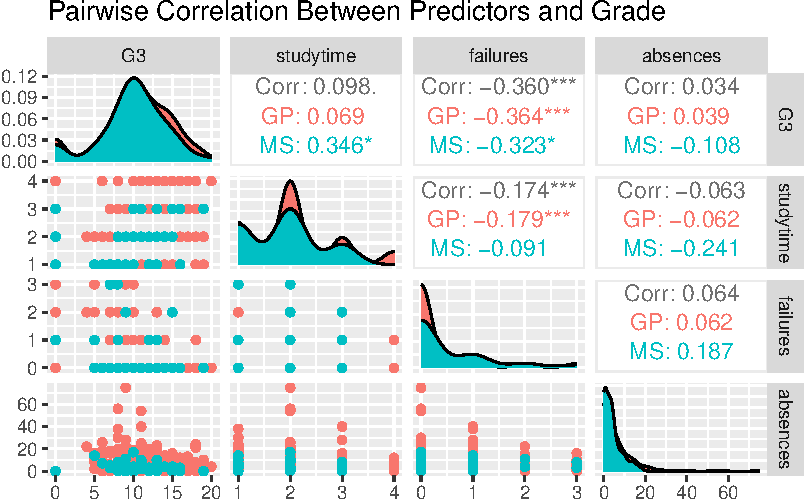
\includegraphics{551-HW-Q3_files/figure-pdf/unnamed-chunk-1-1.pdf}

\begin{Shaded}
\begin{Highlighting}[]
\CommentTok{\# Interaction between gender, studytime, and grade}
\FunctionTok{ggplot}\NormalTok{(d1, }\FunctionTok{aes}\NormalTok{(}\AttributeTok{x =}\NormalTok{ studytime, }\AttributeTok{y =}\NormalTok{ G3, }\AttributeTok{color =}\NormalTok{ sex)) }\SpecialCharTok{+}
  \FunctionTok{geom\_smooth}\NormalTok{(}\AttributeTok{method =} \StringTok{"loess"}\NormalTok{, }\AttributeTok{se =} \ConstantTok{FALSE}\NormalTok{) }\SpecialCharTok{+}
  \FunctionTok{labs}\NormalTok{(}\AttributeTok{title =} \StringTok{"Interaction Between Study Time and Grade by Gender"}\NormalTok{, }
       \AttributeTok{x =} \StringTok{"Study Time"}\NormalTok{, }\AttributeTok{y =} \StringTok{"Final Grade"}\NormalTok{)}
\end{Highlighting}
\end{Shaded}

\begin{verbatim}
`geom_smooth()` using formula = 'y ~ x'
\end{verbatim}

\begin{verbatim}
Warning in simpleLoess(y, x, w, span, degree = degree, parametric = parametric,
: pseudoinverse used at 0.985
\end{verbatim}

\begin{verbatim}
Warning in simpleLoess(y, x, w, span, degree = degree, parametric = parametric,
: neighborhood radius 2.015
\end{verbatim}

\begin{verbatim}
Warning in simpleLoess(y, x, w, span, degree = degree, parametric = parametric,
: reciprocal condition number 6.0033e-16
\end{verbatim}

\begin{verbatim}
Warning in simpleLoess(y, x, w, span, degree = degree, parametric = parametric,
: There are other near singularities as well. 4.0602
\end{verbatim}

\begin{verbatim}
Warning in simpleLoess(y, x, w, span, degree = degree, parametric = parametric,
: pseudoinverse used at 0.985
\end{verbatim}

\begin{verbatim}
Warning in simpleLoess(y, x, w, span, degree = degree, parametric = parametric,
: neighborhood radius 1.015
\end{verbatim}

\begin{verbatim}
Warning in simpleLoess(y, x, w, span, degree = degree, parametric = parametric,
: reciprocal condition number 1.4607e-30
\end{verbatim}

\begin{verbatim}
Warning in simpleLoess(y, x, w, span, degree = degree, parametric = parametric,
: There are other near singularities as well. 1
\end{verbatim}

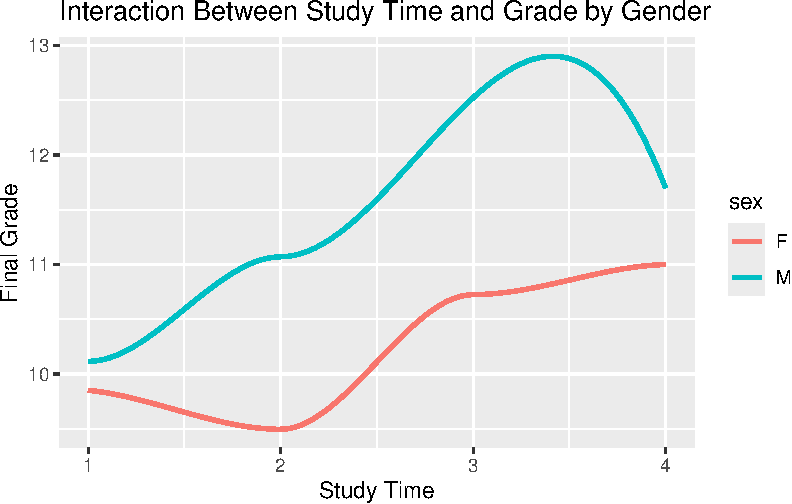
\includegraphics{551-HW-Q3_files/figure-pdf/unnamed-chunk-2-1.pdf}

\begin{Shaded}
\begin{Highlighting}[]
\CommentTok{\# Interaction model}
\NormalTok{interaction\_model }\OtherTok{\textless{}{-}} \FunctionTok{lm}\NormalTok{(G3 }\SpecialCharTok{\textasciitilde{}}\NormalTok{ studytime }\SpecialCharTok{*}\NormalTok{ sex }\SpecialCharTok{+}\NormalTok{ failures }\SpecialCharTok{+}\NormalTok{ absences, }\AttributeTok{data =}\NormalTok{ d1)}

\CommentTok{\# Model summary}
\FunctionTok{summary}\NormalTok{(interaction\_model)}
\end{Highlighting}
\end{Shaded}

\begin{verbatim}

Call:
lm(formula = G3 ~ studytime * sex + failures + absences, data = d1)

Residuals:
     Min       1Q   Median       3Q      Max 
-12.5514  -1.9246   0.2956   2.9146   9.4412 

Coefficients:
               Estimate Std. Error t value Pr(>|t|)    
(Intercept)     9.28052    0.93682   9.906  < 2e-16 ***
studytime       0.47985    0.37384   1.284    0.200    
sexM            1.41074    1.17328   1.202    0.230    
failures       -2.19830    0.29330  -7.495 4.51e-13 ***
absences        0.04153    0.02690   1.544    0.123    
studytime:sexM -0.01480    0.53751  -0.028    0.978    
---
Signif. codes:  0 '***' 0.001 '**' 0.01 '*' 0.05 '.' 0.1 ' ' 1

Residual standard error: 4.238 on 389 degrees of freedom
Multiple R-squared:  0.1551,    Adjusted R-squared:  0.1442 
F-statistic: 14.28 on 5 and 389 DF,  p-value: 7.603e-13
\end{verbatim}

\begin{Shaded}
\begin{Highlighting}[]
\CommentTok{\# Hierarchical model with varying slopes}
\NormalTok{advanced\_hierarchical\_model }\OtherTok{\textless{}{-}} \FunctionTok{stan\_glmer}\NormalTok{(}
\NormalTok{  G3 }\SpecialCharTok{\textasciitilde{}}\NormalTok{ studytime }\SpecialCharTok{+}\NormalTok{ failures }\SpecialCharTok{+}\NormalTok{ absences }\SpecialCharTok{+}\NormalTok{ (}\DecValTok{0} \SpecialCharTok{+}\NormalTok{ studytime }\SpecialCharTok{|}\NormalTok{ school) }\SpecialCharTok{+}\NormalTok{ (}\DecValTok{0} \SpecialCharTok{+} \DecValTok{1} \SpecialCharTok{|}\NormalTok{ sex),}
  \AttributeTok{data =}\NormalTok{ d1,}
  \AttributeTok{family =} \FunctionTok{gaussian}\NormalTok{(),}
  \AttributeTok{prior\_intercept =} \FunctionTok{normal}\NormalTok{(}\DecValTok{10}\NormalTok{, }\DecValTok{2}\NormalTok{),}
  \AttributeTok{prior =} \FunctionTok{normal}\NormalTok{(}\DecValTok{0}\NormalTok{, }\DecValTok{1}\NormalTok{),}
  \AttributeTok{prior\_aux =} \FunctionTok{cauchy}\NormalTok{(}\DecValTok{0}\NormalTok{, }\FloatTok{2.5}\NormalTok{),}
  \AttributeTok{chains =} \DecValTok{4}\NormalTok{,}
  \AttributeTok{iter =} \DecValTok{4000}\NormalTok{,}
  \AttributeTok{seed =} \DecValTok{123}\NormalTok{,}
  \AttributeTok{control =} \FunctionTok{list}\NormalTok{(}\AttributeTok{adapt\_delta =} \FloatTok{0.99}\NormalTok{,}\AttributeTok{max\_treedepth =} \DecValTok{15}\NormalTok{)}

\NormalTok{)}
\end{Highlighting}
\end{Shaded}

\begin{verbatim}
Warning: There were 122 divergent transitions after warmup. See
https://mc-stan.org/misc/warnings.html#divergent-transitions-after-warmup
to find out why this is a problem and how to eliminate them.
\end{verbatim}

\begin{verbatim}
Warning: Examine the pairs() plot to diagnose sampling problems
\end{verbatim}

\begin{Shaded}
\begin{Highlighting}[]
\CommentTok{\# Model summary}
\FunctionTok{summary}\NormalTok{(advanced\_hierarchical\_model)}
\end{Highlighting}
\end{Shaded}

\begin{verbatim}

Model Info:
 function:     stan_glmer
 family:       gaussian [identity]
 formula:      G3 ~ studytime + failures + absences + (0 + studytime | school) + 
       (0 + 1 | sex)
 algorithm:    sampling
 sample:       8000 (posterior sample size)
 priors:       see help('prior_summary')
 observations: 395
 groups:       school (2), sex (2)

Estimates:
                                     mean   sd   10%   50%   90%
(Intercept)                         9.9    1.3  8.3   9.9  11.4 
studytime                           0.4    0.5 -0.2   0.4   0.9 
failures                           -2.0    0.3 -2.4  -2.0  -1.7 
absences                            0.0    0.0  0.0   0.0   0.1 
b[studytime school:GP]              0.1    0.4 -0.4   0.0   0.6 
b[studytime school:MS]              0.2    0.5 -0.3   0.1   0.8 
b[(Intercept) sex:F]               -0.5    1.2 -1.9  -0.5   0.8 
b[(Intercept) sex:M]                0.7    1.2 -0.5   0.6   2.1 
sigma                               4.2    0.2  4.0   4.2   4.4 
Sigma[school:studytime,studytime]   2.4    9.8  0.0   0.2   4.0 
Sigma[sex:(Intercept),(Intercept)]  8.5   24.0  0.3   2.2  18.6 

Fit Diagnostics:
           mean   sd   10%   50%   90%
mean_PPD 10.4    0.3 10.0  10.4  10.8 

The mean_ppd is the sample average posterior predictive distribution of the outcome variable (for details see help('summary.stanreg')).

MCMC diagnostics
                                   mcse Rhat n_eff
(Intercept)                        0.0  1.0  3506 
studytime                          0.0  1.0  1854 
failures                           0.0  1.0  7354 
absences                           0.0  1.0  7018 
b[studytime school:GP]             0.0  1.0  1651 
b[studytime school:MS]             0.0  1.0  1343 
b[(Intercept) sex:F]               0.0  1.0  3018 
b[(Intercept) sex:M]               0.0  1.0  2945 
sigma                              0.0  1.0  5406 
Sigma[school:studytime,studytime]  0.7  1.0   190 
Sigma[sex:(Intercept),(Intercept)] 0.7  1.0  1046 
mean_PPD                           0.0  1.0  7697 
log-posterior                      0.1  1.0  1853 

For each parameter, mcse is Monte Carlo standard error, n_eff is a crude measure of effective sample size, and Rhat is the potential scale reduction factor on split chains (at convergence Rhat=1).
\end{verbatim}

\begin{Shaded}
\begin{Highlighting}[]
\FunctionTok{pairs}\NormalTok{(advanced\_hierarchical\_model, }
      \AttributeTok{pars =} \FunctionTok{c}\NormalTok{(}\StringTok{"(Intercept)"}\NormalTok{, }\StringTok{"studytime"}\NormalTok{, }\StringTok{"failures"}\NormalTok{, }\StringTok{"absences"}\NormalTok{, }\StringTok{"sigma"}\NormalTok{), }
      \AttributeTok{pch =} \DecValTok{20}\NormalTok{,}
      \AttributeTok{cex =} \FloatTok{0.4}\NormalTok{)}
\end{Highlighting}
\end{Shaded}

\begin{verbatim}
Warning: The following arguments were unrecognized and ignored: pch, cex
\end{verbatim}

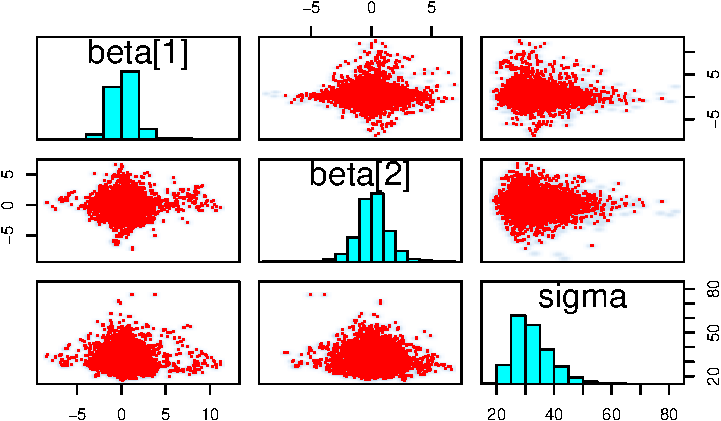
\includegraphics{551-HW-Q3_files/figure-pdf/unnamed-chunk-5-1.pdf}

\begin{Shaded}
\begin{Highlighting}[]
\FunctionTok{summary}\NormalTok{(advanced\_hierarchical\_model)}
\end{Highlighting}
\end{Shaded}

\begin{verbatim}

Model Info:
 function:     stan_glmer
 family:       gaussian [identity]
 formula:      G3 ~ studytime + failures + absences + (0 + studytime | school) + 
       (0 + 1 | sex)
 algorithm:    sampling
 sample:       8000 (posterior sample size)
 priors:       see help('prior_summary')
 observations: 395
 groups:       school (2), sex (2)

Estimates:
                                     mean   sd   10%   50%   90%
(Intercept)                         9.9    1.3  8.3   9.9  11.4 
studytime                           0.4    0.5 -0.2   0.4   0.9 
failures                           -2.0    0.3 -2.4  -2.0  -1.7 
absences                            0.0    0.0  0.0   0.0   0.1 
b[studytime school:GP]              0.1    0.4 -0.4   0.0   0.6 
b[studytime school:MS]              0.2    0.5 -0.3   0.1   0.8 
b[(Intercept) sex:F]               -0.5    1.2 -1.9  -0.5   0.8 
b[(Intercept) sex:M]                0.7    1.2 -0.5   0.6   2.1 
sigma                               4.2    0.2  4.0   4.2   4.4 
Sigma[school:studytime,studytime]   2.4    9.8  0.0   0.2   4.0 
Sigma[sex:(Intercept),(Intercept)]  8.5   24.0  0.3   2.2  18.6 

Fit Diagnostics:
           mean   sd   10%   50%   90%
mean_PPD 10.4    0.3 10.0  10.4  10.8 

The mean_ppd is the sample average posterior predictive distribution of the outcome variable (for details see help('summary.stanreg')).

MCMC diagnostics
                                   mcse Rhat n_eff
(Intercept)                        0.0  1.0  3506 
studytime                          0.0  1.0  1854 
failures                           0.0  1.0  7354 
absences                           0.0  1.0  7018 
b[studytime school:GP]             0.0  1.0  1651 
b[studytime school:MS]             0.0  1.0  1343 
b[(Intercept) sex:F]               0.0  1.0  3018 
b[(Intercept) sex:M]               0.0  1.0  2945 
sigma                              0.0  1.0  5406 
Sigma[school:studytime,studytime]  0.7  1.0   190 
Sigma[sex:(Intercept),(Intercept)] 0.7  1.0  1046 
mean_PPD                           0.0  1.0  7697 
log-posterior                      0.1  1.0  1853 

For each parameter, mcse is Monte Carlo standard error, n_eff is a crude measure of effective sample size, and Rhat is the potential scale reduction factor on split chains (at convergence Rhat=1).
\end{verbatim}

\begin{Shaded}
\begin{Highlighting}[]
\NormalTok{posterior\_summary }\OtherTok{\textless{}{-}} \FunctionTok{as.data.frame}\NormalTok{(}\FunctionTok{posterior\_interval}\NormalTok{(advanced\_hierarchical\_model))}
\FunctionTok{print}\NormalTok{(posterior\_summary)}
\end{Highlighting}
\end{Shaded}

\begin{verbatim}
                                             5%         95%
(Intercept)                         7.684803190 11.86183401
studytime                          -0.456541709  1.08684677
failures                           -2.498991945 -1.56764640
absences                           -0.004339904  0.08580278
b[studytime school:GP]             -0.557159194  0.86625736
b[studytime school:MS]             -0.463538850  1.08573242
b[(Intercept) sex:F]               -2.401351131  1.36718496
b[(Intercept) sex:M]               -1.063535685  2.70176240
sigma                               3.989168571  4.49323821
Sigma[school:studytime,studytime]   0.001263832  8.78707645
Sigma[sex:(Intercept),(Intercept)]  0.170298758 33.10170253
\end{verbatim}

\begin{Shaded}
\begin{Highlighting}[]
\CommentTok{\# Global PPC}
\FunctionTok{pp\_check}\NormalTok{(advanced\_hierarchical\_model) }\SpecialCharTok{+}
  \FunctionTok{ggtitle}\NormalTok{(}\StringTok{"Global Posterior Predictive Check for Hierarchical Model"}\NormalTok{)}
\end{Highlighting}
\end{Shaded}

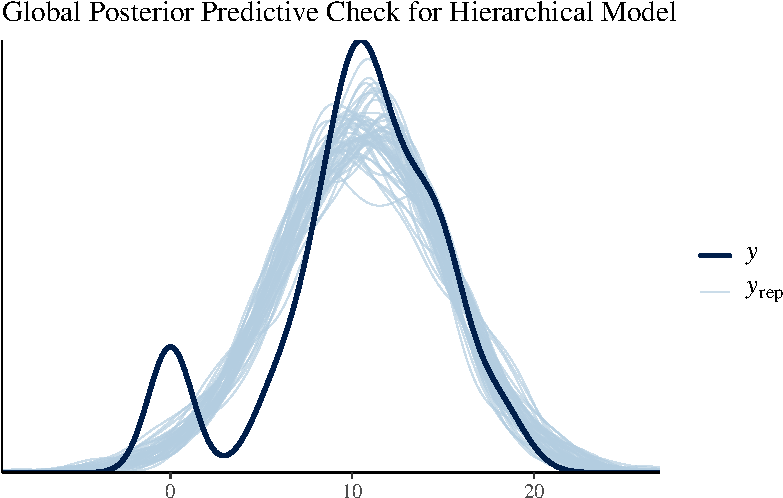
\includegraphics{551-HW-Q3_files/figure-pdf/unnamed-chunk-8-1.pdf}

\begin{Shaded}
\begin{Highlighting}[]
\CommentTok{\# Group{-}level PPC}
\FunctionTok{pp\_check}\NormalTok{(advanced\_hierarchical\_model, }\AttributeTok{group =} \StringTok{"school"}\NormalTok{) }\SpecialCharTok{+}
  \FunctionTok{ggtitle}\NormalTok{(}\StringTok{"Posterior Predictive Check by School"}\NormalTok{)}
\end{Highlighting}
\end{Shaded}

\begin{verbatim}
Warning: The following arguments were unrecognized and ignored: group
\end{verbatim}

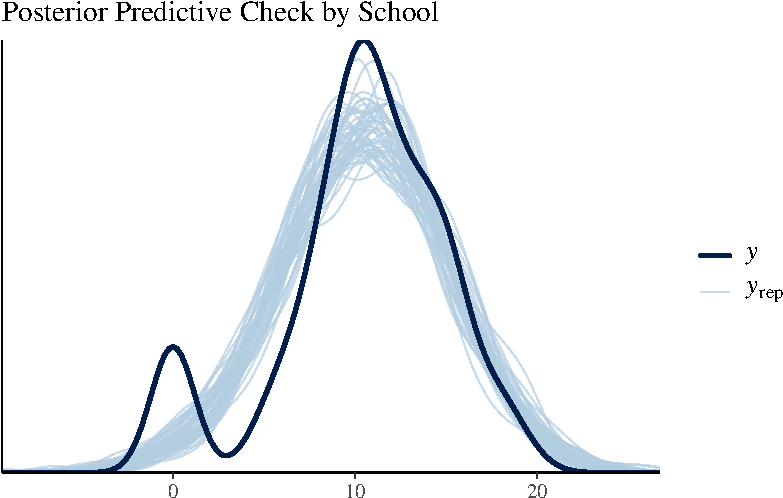
\includegraphics{551-HW-Q3_files/figure-pdf/unnamed-chunk-9-1.pdf}

\begin{Shaded}
\begin{Highlighting}[]
\CommentTok{\# library(shinystan)}
\CommentTok{\# launch\_shinystan(advanced\_hierarchical\_model)}
\end{Highlighting}
\end{Shaded}

\begin{Shaded}
\begin{Highlighting}[]
\CommentTok{\# posterior \textless{}{-} as.matrix(advanced\_hierarchical\_model)}
\CommentTok{\# divergences \textless{}{-} sum(attr(posterior, "sampler\_params")$divergent\_\_)}
\CommentTok{\# print(divergences) }
\end{Highlighting}
\end{Shaded}

\begin{Shaded}
\begin{Highlighting}[]
\CommentTok{\# Install and load rstanarm if needed}
\ControlFlowTok{if}\NormalTok{ (}\SpecialCharTok{!}\FunctionTok{requireNamespace}\NormalTok{(}\StringTok{"rstanarm"}\NormalTok{, }\AttributeTok{quietly =} \ConstantTok{TRUE}\NormalTok{)) }\FunctionTok{install.packages}\NormalTok{(}\StringTok{"rstanarm"}\NormalTok{)}
\FunctionTok{library}\NormalTok{(rstanarm)}

\CommentTok{\# Bayesian interaction model}
\NormalTok{bayesian\_interaction\_model }\OtherTok{\textless{}{-}} \FunctionTok{stan\_glm}\NormalTok{(}
\NormalTok{  G3 }\SpecialCharTok{\textasciitilde{}}\NormalTok{ studytime }\SpecialCharTok{*}\NormalTok{ sex }\SpecialCharTok{+}\NormalTok{ failures }\SpecialCharTok{+}\NormalTok{ absences,}
  \AttributeTok{data =}\NormalTok{ d1,}
  \AttributeTok{family =} \FunctionTok{gaussian}\NormalTok{(),}
  \AttributeTok{prior\_intercept =} \FunctionTok{normal}\NormalTok{(}\DecValTok{10}\NormalTok{, }\DecValTok{5}\NormalTok{),}
  \AttributeTok{prior =} \FunctionTok{normal}\NormalTok{(}\DecValTok{0}\NormalTok{, }\FloatTok{2.5}\NormalTok{),}
  \AttributeTok{prior\_aux =} \FunctionTok{cauchy}\NormalTok{(}\DecValTok{0}\NormalTok{, }\DecValTok{2}\NormalTok{),}
  \AttributeTok{chains =} \DecValTok{4}\NormalTok{,}
  \AttributeTok{iter =} \DecValTok{2000}\NormalTok{,}
  \AttributeTok{seed =} \DecValTok{123}
\NormalTok{)}
\end{Highlighting}
\end{Shaded}

\begin{Shaded}
\begin{Highlighting}[]
\CommentTok{\# Compute WAIC for the Bayesian models}
\NormalTok{waic\_one\_param }\OtherTok{\textless{}{-}} \FunctionTok{waic}\NormalTok{(bayesian\_interaction\_model)}
\end{Highlighting}
\end{Shaded}

\begin{verbatim}
Warning: 
1 (0.3%) p_waic estimates greater than 0.4. We recommend trying loo instead.
\end{verbatim}

\begin{Shaded}
\begin{Highlighting}[]
\NormalTok{waic\_hierarchical }\OtherTok{\textless{}{-}} \FunctionTok{waic}\NormalTok{(advanced\_hierarchical\_model)}

\CommentTok{\# Print WAIC results}
\FunctionTok{print}\NormalTok{(waic\_one\_param)}
\end{Highlighting}
\end{Shaded}

\begin{verbatim}

Computed from 4000 by 395 log-likelihood matrix.

          Estimate   SE
elpd_waic  -1135.0 15.7
p_waic         7.2  0.8
waic        2270.0 31.4

1 (0.3%) p_waic estimates greater than 0.4. We recommend trying loo instead. 
\end{verbatim}

\begin{Shaded}
\begin{Highlighting}[]
\FunctionTok{print}\NormalTok{(waic\_hierarchical)}
\end{Highlighting}
\end{Shaded}

\begin{verbatim}

Computed from 8000 by 395 log-likelihood matrix.

          Estimate   SE
elpd_waic  -1134.9 15.7
p_waic         7.1  0.7
waic        2269.9 31.4
\end{verbatim}

\begin{Shaded}
\begin{Highlighting}[]
\CommentTok{\# Compute LOO for both models}
\NormalTok{loo\_one\_param }\OtherTok{\textless{}{-}} \FunctionTok{loo}\NormalTok{(bayesian\_interaction\_model)}
\NormalTok{loo\_hierarchical }\OtherTok{\textless{}{-}} \FunctionTok{loo}\NormalTok{(advanced\_hierarchical\_model)}

\CommentTok{\# Compare models using loo\_compare}
\NormalTok{loo\_comparison }\OtherTok{\textless{}{-}} \FunctionTok{loo\_compare}\NormalTok{(loo\_one\_param, loo\_hierarchical)}

\CommentTok{\# Print LOO comparison results}
\FunctionTok{print}\NormalTok{(loo\_comparison)}
\end{Highlighting}
\end{Shaded}

\begin{verbatim}
                            elpd_diff se_diff
advanced_hierarchical_model  0.0       0.0   
bayesian_interaction_model  -0.1       0.8   
\end{verbatim}

\begin{Shaded}
\begin{Highlighting}[]
\CommentTok{\# Posterior predictive checks for the interaction model}
\FunctionTok{pp\_check}\NormalTok{(bayesian\_interaction\_model)}
\end{Highlighting}
\end{Shaded}

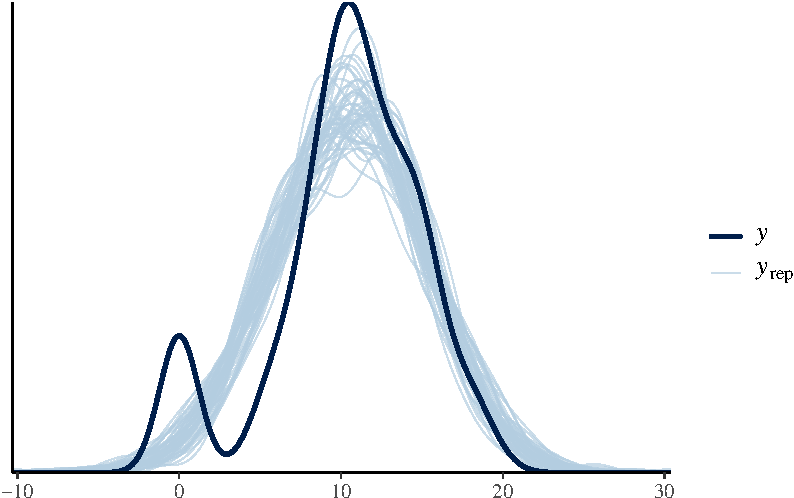
\includegraphics{551-HW-Q3_files/figure-pdf/unnamed-chunk-15-1.pdf}

\begin{Shaded}
\begin{Highlighting}[]
\CommentTok{\# Posterior predictive checks for the hierarchical model}
\FunctionTok{pp\_check}\NormalTok{(advanced\_hierarchical\_model)}
\end{Highlighting}
\end{Shaded}

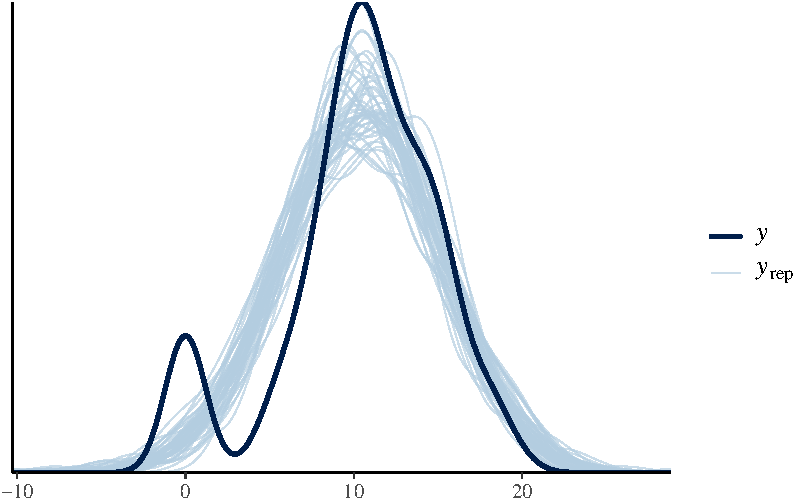
\includegraphics{551-HW-Q3_files/figure-pdf/unnamed-chunk-15-2.pdf}

\begin{Shaded}
\begin{Highlighting}[]
\CommentTok{\# Extract posterior samples for random effects}
\FunctionTok{library}\NormalTok{(bayesplot)}
\end{Highlighting}
\end{Shaded}

\begin{verbatim}
This is bayesplot version 1.11.1
\end{verbatim}

\begin{verbatim}
- Online documentation and vignettes at mc-stan.org/bayesplot
\end{verbatim}

\begin{verbatim}
- bayesplot theme set to bayesplot::theme_default()
\end{verbatim}

\begin{verbatim}
   * Does _not_ affect other ggplot2 plots
\end{verbatim}

\begin{verbatim}
   * See ?bayesplot_theme_set for details on theme setting
\end{verbatim}

\begin{Shaded}
\begin{Highlighting}[]
\NormalTok{posterior\_samples }\OtherTok{\textless{}{-}} \FunctionTok{as.data.frame}\NormalTok{(advanced\_hierarchical\_model)}

\FunctionTok{colnames}\NormalTok{(posterior\_samples) }\CommentTok{\# List all parameter names}
\end{Highlighting}
\end{Shaded}

\begin{verbatim}
 [1] "(Intercept)"                        "studytime"                         
 [3] "failures"                           "absences"                          
 [5] "b[studytime school:GP]"             "b[studytime school:MS]"            
 [7] "b[(Intercept) sex:F]"               "b[(Intercept) sex:M]"              
 [9] "sigma"                              "Sigma[school:studytime,studytime]" 
[11] "Sigma[sex:(Intercept),(Intercept)]"
\end{verbatim}

\begin{Shaded}
\begin{Highlighting}[]
\CommentTok{\# Visualize posterior for group{-}level intercepts (schools)}
\FunctionTok{mcmc\_areas}\NormalTok{(}
\NormalTok{  posterior\_samples,}
  \AttributeTok{pars =} \FunctionTok{c}\NormalTok{(}\StringTok{"b[studytime school:GP]"}\NormalTok{, }\StringTok{"b[studytime school:MS]"}\NormalTok{),}
  \AttributeTok{prob =} \FloatTok{0.8}
\NormalTok{) }\SpecialCharTok{+}
  \FunctionTok{labs}\NormalTok{(}
    \AttributeTok{title =} \StringTok{"Posterior Distributions for School{-}Level Effects"}\NormalTok{,}
    \AttributeTok{x =} \StringTok{"Effect Size"}\NormalTok{,}
    \AttributeTok{y =} \StringTok{"Density"}
\NormalTok{  )}
\end{Highlighting}
\end{Shaded}

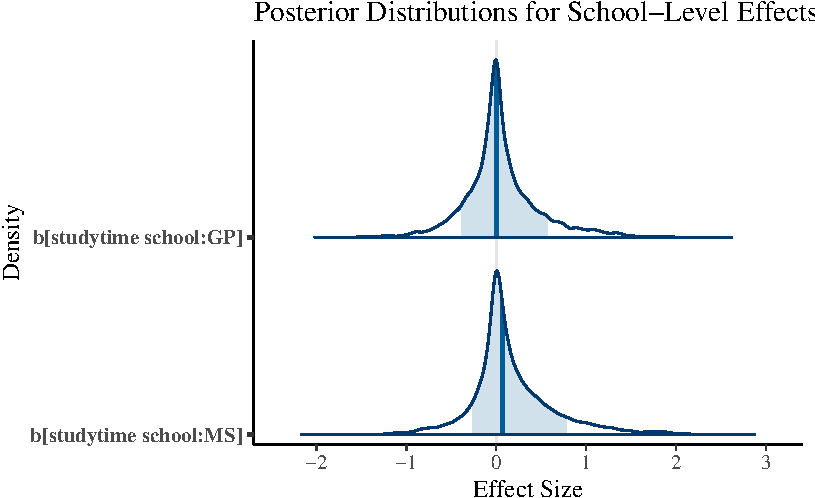
\includegraphics{551-HW-Q3_files/figure-pdf/unnamed-chunk-16-1.pdf}

\begin{center}\rule{0.5\linewidth}{0.5pt}\end{center}




\end{document}
